% THIS IS SIGPROC-SP.TEX - VERSION 3.1
% WORKS WITH V3.2SP OF ACM_PROC_ARTICLE-SP.CLS
% APRIL 2009
%
% It is an example file showing how to use the 'acm_proc_article-sp.cls' V3.2SP
% LaTeX2e document class file for Conference Proceedings submissions.
% ----------------------------------------------------------------------------------------------------------------
% This .tex file (and associated .cls V3.2SP) *DOES NOT* produce:
%       1) The Permission Statement
%       2) The Conference (location) Info information
%       3) The Copyright Line with ACM data
%       4) Page numbering
% ---------------------------------------------------------------------------------------------------------------
% It is an example which *does* use the .bib file (from which the .bbl file
% is produced).
% REMEMBER HOWEVER: After having produced the .bbl file,
% and prior to final submission,
% you need to 'insert'  your .bbl file into your source .tex file so as to provide
% ONE 'self-contained' source file.
%
% Questions regarding SIGS should be sent to
% Adrienne Griscti ---> griscti@acm.org
%
% Questions/suggestions regarding the guidelines, .tex and .cls files, etc. to
% Gerald Murray ---> murray@hq.acm.org
%
% For tracking purposes - this is V3.1SP - APRIL 2009

%Old document Class 
%\documentclass[a4paper]{acm_proc_article-sp}
\documentclass{sig-alternate}
%\usepackage[margin=1in]{geometry}
\usepackage{amsmath}
\usepackage{url}
\usepackage{graphicx}
\usepackage{alltt}
\usepackage{algorithm}

\usepackage{algorithmic}
\usepackage{cite}
\usepackage{flushend}
\usepackage{tabularx}

%\lstset{language=C}
\usepackage{times}
\usepackage{graphicx}
\usepackage{epsf}
\usepackage{verbatim}
\usepackage{psfig}
\usepackage{cite}
\usepackage{url}
\usepackage{color}
\usepackage[table]{xcolor}
\usepackage{booktabs, dcolumn}
\usepackage{alltt}

\usepackage{longtable,lscape}
\usepackage{slashbox,multirow}
\usepackage{colortbl}
\usepackage{mathrsfs}

\newcommand{\Add}{\CodeIn{add}}
\newcommand{\AVTree}{\CodeIn{AVTree}}
\newcommand{\Assignment}[3]{$\langle$ \Object{#1}, \Object{#2}, \Object{#3} $\rangle$}
\newcommand{\BinaryTreeRemove}{\CodeIn{BinaryTree\_remove}}
\newcommand{\BinaryTree}{\CodeIn{BinaryTree}}
\newcommand{\Caption}{\caption}
\newcommand{\Char}[1]{`#1'}
\newcommand{\CheckRep}{\CodeIn{checkRep}}
\newcommand{\ClassC}{\CodeIn{C}}
\newcommand{\CodeIn}[1]{{\small\texttt{#1}}}
\newcommand{\CodeOutSize}{\scriptsize}
\newcommand{\Comment}[1]{}
\newcommand{\Ensures}{\CodeIn{ensures}}
\newcommand{\ExtractMax}{\CodeIn{extractMax}}
\newcommand{\FAL}{field-ordering}
\newcommand{\FALs}{field-orderings}
\newcommand{\Fact}{observation}
\newcommand{\Get}{\CodeIn{get}}
\newcommand{\HashSet}{\CodeIn{HashSet}}
\newcommand{\HeapArray}{\CodeIn{HeapArray}}
\newcommand{\Intro}[1]{\emph{#1}}
\newcommand{\Invariant}{\CodeIn{invariant}}
\newcommand{\JUC}{\CodeIn{java.\-util.\-Collections}}
\newcommand{\JUS}{\CodeIn{java.\-util.\-Set}}
\newcommand{\JUTM}{\CodeIn{java.\-util.\-TreeMap}}
\newcommand{\JUTS}{\CodeIn{java.\-util.\-TreeSet}}
\newcommand{\JUV}{\CodeIn{java.\-util.\-Vector}}
\newcommand{\JMLPlusJUnit}{JML+JUnit}
\newcommand{\Korat}{Korat}
\newcommand{\Left}{\CodeIn{left}}
\newcommand{\Lookup}{\CodeIn{lookup}}
\newcommand{\MethM}{\CodeIn{m}}
\newcommand{\Node}[1]{\CodeIn{N}$_#1$}
\newcommand{\Null}{\CodeIn{null}}
\newcommand{\Object}[1]{\CodeIn{o}\ensuremath{_#1}}
\newcommand{\PostM}{\MethM$_{post}$}
\newcommand{\PreM}{\MethM$_{pre}$}
\newcommand{\Put}{\CodeIn{put}}
\newcommand{\Remove}{\CodeIn{remove}}
\newcommand{\RepOk}{\CodeIn{repOk}}
\newcommand{\Requires}{\CodeIn{requires}}
\newcommand{\Reverse}{\CodeIn{reverse}}
\newcommand{\Right}{\CodeIn{right}}
\newcommand{\Root}{\CodeIn{root}}
\newcommand{\Set}{\CodeIn{set}}
\newcommand{\State}[1]{2^{#1}}
\newcommand{\TestEra}{TestEra}
\newcommand{\TreeMap}{\CodeIn{TreeMap}}

\newenvironment{CodeOut}{\begin{scriptsize}}{\end{scriptsize}}
\newenvironment{SmallOut}{\begin{small}}{\end{small}}

\newcommand{\pairwiseEquals}{PairwiseEquals}
\newcommand{\monitorEquals}{MonitorEquals}
%\newcommand{\monitorWField}{WholeStateW}
\newcommand{\traverseField}{WholeState}
\newcommand{\monitorSMSeq}{ModifyingSeq}
\newcommand{\monitorSeq}{WholeSeq}

\newcommand{\IntStack}{\CodeIn{IntStack}}
\newcommand{\UBStack}{\CodeIn{UBStack}}
\newcommand{\BSet}{\CodeIn{BSet}}
\newcommand{\BBag}{\CodeIn{BBag}}
\newcommand{\ShoppingCart}{\CodeIn{ShoppingCart}}
\newcommand{\BankAccount}{\CodeIn{BankAccount}}
\newcommand{\BinarySearchTree}{\CodeIn{BinarySearchTree}}
\newcommand{\LinkedList}{\CodeIn{LinkedList}}

\newcommand{\Book}{\CodeIn{Book}}
\newcommand{\Library}{\CodeIn{Library}}

\newcommand{\Jtest}{Jtest}
\newcommand{\JCrasher}{JCrasher}
\newcommand{\Daikon}{Daikon}
\newcommand{\JUnit}{JUnit}

\newcommand{\trie}{trie}

\newcommand{\Perl}{Perl}


\newcommand{\SubjectCount}{11}
\newcommand{\DSSubjectCount}{two}

\newcommand{\Equals}{\CodeIn{equals}}
\newcommand{\Pairwise}{PairwiseEquals}
\newcommand{\Subgraph}{MonitorEquals}
\newcommand{\Concrete}{WholeState}
\newcommand{\ModSeq}{ModifyingSeq}
\newcommand{\Seq}{WholeSeq}
\newcommand{\Aeq}{equality}

\newcommand{\Meaning}[1]{\ensuremath{[\![}#1\ensuremath{]\!]}}
\newcommand{\Pair}[2]{\ensuremath{\langle #1, #2 \rangle}}
\newcommand{\Triple}[3]{\ensuremath{\langle #1, #2, #3 \rangle}}
\newcommand{\SetSuch}[2]{\ensuremath{\{ #1 | #2 \}}}

\newcommand{\Equiv}[2]{\ensuremath{#1 \EquivSTRel{} #2}}
\newcommand{\EquivME}{\Equiv}
\newcommand{\EquivST}{\Equiv}
\newcommand{\EquivSTRel}{\ensuremath{\cong}}
\newcommand{\Redundant}[2]{\ensuremath{#1 \lhd #2}}
\newcommand{\VB}{\ensuremath{\mid}}
\newcommand{\MES}{method-entry state}

\newcommand{\Small}[1]{{\small{#1}}}

\newcommand{\CenterCell}[1]{\multicolumn{1}{c|}{#1}}

% Yoonki's code
\colorlet{tableheadcolor}{gray!25} % Table header colour = 25% gray
\newcommand{\headcol}{\rowcolor{tableheadcolor}} %
\colorlet{tablerowcolor}{gray!10} % Table row separator colour = 10% gray
\newcommand{\rowcol}{\rowcolor{tablerowcolor}} %
    % Command \topline consists of a (slightly modified) \toprule followed by a \heavyrule rule of colour tableheadcolor (hence, 2 separate rules)
\newcommand{\topline}{\arrayrulecolor{black}\specialrule{0.1em}{\abovetopsep}{0pt}%
            \arrayrulecolor{tableheadcolor}\specialrule{\belowrulesep}{0pt}{0pt}%
            \arrayrulecolor{black}}
    % Command \midline consists of 3 rules (top colour tableheadcolor, middle colour black, bottom colour white)
\newcommand{\midline}{\arrayrulecolor{tableheadcolor}\specialrule{\aboverulesep}{0pt}{0pt}%
            \arrayrulecolor{black}\specialrule{\lightrulewidth}{0pt}{0pt}%
            \arrayrulecolor{white}\specialrule{\belowrulesep}{0pt}{0pt}%
            \arrayrulecolor{black}}
    % Command \rowmidlinecw consists of 3 rules (top colour tablerowcolor, middle colour black, bottom colour white)
\newcommand{\rowmidlinecw}{\arrayrulecolor{tablerowcolor}\specialrule{\aboverulesep}{0pt}{0pt}%
            \arrayrulecolor{black}\specialrule{\lightrulewidth}{0pt}{0pt}%
            \arrayrulecolor{white}\specialrule{\belowrulesep}{0pt}{0pt}%
            \arrayrulecolor{black}}
    % Command \rowmidlinewc consists of 3 rules (top colour white, middle colour black, bottom colour tablerowcolor)
\newcommand{\rowmidlinewc}{\arrayrulecolor{white}\specialrule{\aboverulesep}{0pt}{0pt}%
            \arrayrulecolor{black}\specialrule{\lightrulewidth}{0pt}{0pt}%
            \arrayrulecolor{tablerowcolor}\specialrule{\belowrulesep}{0pt}{0pt}%
            \arrayrulecolor{black}}
    % Command \rowmidlinew consists of 1 white rule
\newcommand{\rowmidlinew}{\arrayrulecolor{white}\specialrule{\aboverulesep}{0pt}{0pt}%
            \arrayrulecolor{black}}
    % Command \rowmidlinec consists of 1 tablerowcolor rule
\newcommand{\rowmidlinec}{\arrayrulecolor{tablerowcolor}\specialrule{\aboverulesep}{0pt}{0pt}%
            \arrayrulecolor{black}}
    % Command \bottomline consists of 2 rules (top colour
\newcommand{\bottomline}{\arrayrulecolor{white}\specialrule{\aboverulesep}{0pt}{0pt}%
            \arrayrulecolor{black}\specialrule{\heavyrulewidth}{0pt}{\belowbottomsep}}%
\newcommand{\bottomlinec}{\arrayrulecolor{tablerowcolor}\specialrule{\aboverulesep}{0pt}{0pt}%
            \arrayrulecolor{black}\specialrule{\heavyrulewidth}{0pt}{\belowbottomsep}}%


\addtolength{\topmargin}{.825in}

\newcommand{\tool}{{\sc ICON}}
\newcommand{\amazon}{\CodeIn{Amazon S3 REST API} developer documentation}
\newcommand{\amazonAPI}{\CodeIn{Amazon S3 REST API}}


\begin{document}
%
% --- Author Metadata here ---
\conferenceinfo{FSE}{'14 Hong Kong}
%\CopyrightYear{2007} % Allows default copyright year (20XX) to be over-ridden - IF NEED BE.
%\crdata{0-12345-67-8/90/01}  % Allows default copyright data (0-89791-88-6/97/05) to be over-ridden - IF NEED BE.
% --- End of Author Metadata ---

\title{{\ttlit ICON}: {\ttlit I}nferring Temporal {\ttlit Con}straints from Natural Language API Descriptions}
%\subtitle{[Extended Abstract]
%\titlenote{A full version of this paper is available as
%\textit{Author's Guide to Preparing ACM SIG Proceedings Using
%\LaTeX$2_\epsilon$\ and BibTeX} at
%\texttt{www.acm.org/eaddress.htm}}}
%
% You need the command \numberofauthors to handle the 'placement
% and alignment' of the authors beneath the title.
%
% For aesthetic reasons, we recommend 'three authors at a time'
% i.e. three 'name/affiliation blocks' be placed beneath the title.
%
% NOTE: You are NOT restricted in how many 'rows' of
% "name/affiliations" may appear. We just ask that you restrict
% the number of 'columns' to three.
%
% Because of the available 'opening page real-estate'
% we ask you to refrain from putting more than six authors
% (two rows with three columns) beneath the article title.
% More than six makes the first-page appear very cluttered indeed.
%
% Use the \alignauthor commands to handle the names
% and affiliations for an 'aesthetic maximum' of six authors.
% Add names, affiliations, addresses for
% the seventh etc. author(s) as the argument for the
% \additionalauthors command.
% These 'additional authors' will be output/set for you
% without further effort on your part as the last section in
% the body of your article BEFORE References or any Appendices.

\numberofauthors{1} %  in this sample file, there are a *total*
% of EIGHT authors. SIX appear on the 'first-page' (for formatting
% reasons) and the remaining two appear in the \additionalauthors section.
%
\author{
% You can go ahead and credit any number of authors here,
% e.g. one 'row of three' or two rows (consisting of one row of three
% and a second row of one, two or three).
%
% The command \alignauthor (no curly braces needed) should
% precede each author name, affiliation/snail-mail address and
% e-mail address. Additionally, tag each line of
% affiliation/address with \affaddr, and tag the
% e-mail address with \email.
%
% 1st. author
\alignauthor
Rahul Pandita$^1$, Kunal Taneja$^2$, Tao Xie$^3$, Laurie Williams$^1$, Teresa Tung$^2$\\%\titlenote{Dr.~Trovato insisted his name be first.}\\
       \affaddr{$^1$Department of Computer Science, North Carolina State University, Raleigh, NC, USA}\\
       \affaddr{$^2$Accenture Technology Labs, San Jose, CA, USA}\\
       \affaddr{$^3$Department of Computer Science, University of Illinois, Urbana-Champaign, IL, USA}\\
       \email{{\normalsize rpandit@ncsu.edu, k.a.taneja@accenture.com, taoxie@illinois.edu, williams@csc.ncsu.edu, teresa.tung@accenture.com}}
% 2nd. author
%\alignauthor
%Kunal Taneja\\
%	   %\titlenote{The secretary disavows any knowledge of this author's actions.}\\
%       \affaddr{Accenture Technology Labs}\\
%       \affaddr{San Jose, CA, USA}\\
%       \email{k.a.taneja@accenture.com}
%% 3rd. author
%\alignauthor 
%Tao Xie\\
%	   %\titlenote{This author is the one who did all the really hard work.}\\
%       %\affaddr{Department of Computer Science}\\
%       \affaddr{University of Illinois}\\
%       \affaddr{Urbana-Champaign, IL, USA}\\
%       \email{taoxie@illinois.edu}
%\and  % use '\and' if you need 'another row' of author names
%% 4th. author
%\alignauthor Laurie Williams\\
%       %\affaddr{Department of Computer Science}\\
%       \affaddr{North Carolina State University}\\
%       \affaddr{Raleigh, NC, USA}\\
%       \email{williams@csc.ncsu.edu}
%% 5th. author
%\alignauthor Teresa Tung\\
%       \affaddr{Accenture Technology Labs}\\
%       \affaddr{San Jose, CA, USA}\\
%       \email{teresa.tung@accenture.com}
}
% There's nothing stopping you putting the seventh, eighth, etc.
% author on the opening page (as the 'third row') but we ask,
% for aesthetic reasons that you place these 'additional authors'
% in the \additional authors block, viz.
%\additionalauthors{Additional authors: John Smith (The Th{\o}rv{\"a}ld Group,
%email: {\texttt{jsmith@affiliation.org}}) and Julius P.~Kumquat
%(The Kumquat Consortium, email: {\texttt{jpkumquat@consortium.net}}).}
\date{30 July 1999}
% Just remember to make sure that the TOTAL number of authors
% is the number that will appear on the first page PLUS the
% number that will appear in the \additionalauthors section.

\maketitle
\begin{abstract}
Temporal specifications of an Application Programming
Interface (API) describe allowed sequences of invocations
of methods within an API. Despite being desirable for 
software testing and verification (through formal analysis tools),
most API's do not have formal temporal specifications.
In contrast, API documents contain valuable information about the usage in natural language.
However, formal analysis tools are not designed to work on specifications in natural languages.
Manually writing formal specifications based on natural language text in API documents
can be prohibitively time consuming and error prone.
To address this issue, we propose a natural language processing based automated approach \tool ,
to infer formal temporal specifications from natural language text of API documents.
To evaluate our proposed approach, we applied \tool\ to infer temporal constraints from 
commonly used package \CodeIn{java.io} from JDK API and Amazon S3 REST API.
Our evaluation results show that \tool\ achieves an average of 60\% precision and 80\% recall
in inferring 63 temporal constraints from more than 2400 sentences of API documents. 


% need to explain why moving from formal specifications to temporal constraints

% Goal statement
% The goal of this research is to facilitate the correct usage API methods by identifying temporal constraints etc.. 
\end{abstract}

% A category with the (minimum) three required fields
%\category{D.4}{Information Systems Applications}{Miscellaneous}
%A category including the fourth, optional field follows...
%\category{D.2.1}{Software Engineering}{Requirements/Specification}[complexity measures, performance measures]

\category{D.2.1}{Software Engineering}{Requirements/Specifications}
\category{F.3.1}{LOGICS AND MEANINGS OF PROGRAMS}{Specifying and Verifying and Reasoning about Programs} [Specification techniques]
\terms{Specifications}

\keywords{Temporal Specifications, NLP, API Documents} % NOT required for Proceedings

\section{Introduction}
\label{sec:introduction}


Temporal constraints~\cite{ball2002s} of an Application Programming Interface (API) 
are the allowed sequences of invocations of methods from the API. 
These constraints govern the secure and robust operation of client software using the API.
If these constraints are in a formal specification language,
they can be used as inputs to formal analysis tools such 
as model checker and runtime verifiers
in detecting the violations of these temporal constraints as defects~\cite{lee2012towards}.

Typically, temporal constraints are described in natural language text of API documents.
Such documents are provided to client-code developers through an online access, or are shipped with the API code.
For a method under consideration, an API document may describe both the constraints on the method parameters
as well as the temporal constraints in terms of other methods that must be invoked pre/post invoking that method.
We observe that a non-trivial portion (roughly 12\%) of the sentences (constraint-describing sentences)
in \amazonAPI\ documentation describe temporal constraints.
However, existing verification tools, which typically accept only formal constraints,
cannot use the natural language constraints from API documents.

Although natural language API description can be manually converted into formal constraints,
manually writing formal constraints based on natural language text in API documents can be prohibitively time consuming and error prone~\cite{wu2013inferring,RubingerWEB10}. 
For instance, Wu et al.~\cite{wu2013inferring} report that it took one person ten hours to browse the documentation of one method from a web service API, even before the person attempted to formalize the constraints on the method.


To reduce the manual effort, we propose \tool: a Natural Language Processing (NLP) based approach
to automatically infer formal temporal constraints. 
However, inferring temporal constraints from the natural language text is challenging. 
In particular, our approach addresses two major challenges to automatically infer specifications
from natural language text in API documents.

First, existing NLP techniques are initially designed towards well-written news articles.
In contrast, API documents are domain-specific documents and are often not well formed.
Furthermore, we observe that generic NLP techniques face problems with lengthy sentences (with a number of lexical tokens).
Consider the description sentence ``All objects (including all object versions and Delete Markers) in the bucket must be deleted before the bucket itself can be delete.'' The length of the sentence may overwhelm an NLP parser, which then inaccurately extracts semantic relations between the words in the sentence.
Our ICON approach includes a new technique called ``hybrid parsing'' to deal with the number of lexical tokens.
Hybrid parsing automatically breaks lengthy sentences to smaller tractable sentences based on a function of parts-of-speech tags.   

Second, after API documents are made amenable to existing NLP techniques, a method referenced in the natural language text must be identified in order to infer temporal constraints on the method but such method referencing is often implicit.
Consider the description sentence ``You must initiate a multipart upload before you can upload any part.''
In this sentence, phrases ``multipart upload'' and ``upload any part'' refer to individual methods in the API.
Identifying these phrases as method-invocation instances requires domain dictionaries.
Ad-hoc construction of such dictionaries is prohibitively time and resource intensive.
To address this challenge, we propose to build domain dictionaries systematically from API documents and generic English dictionaries.  

In summary, our \tool\ approach leverages natural language description of API's to infer temporal constraints of method invocations.
As our approach analyzes API documents in natural language, it can be reused independent of the programming language of an API library.
Additionally, our approach complements existing mining-based approaches~\cite{buse2012synthesizing, thummalapenta07parseweb, Wang:2013:MSR, Zhong:2009:MMR} that partially address the problem by mining for common usage patterns among client code reusing the API.
This paper makes the following main contributions:
%However, all of these approaches rely on the availability of the source code that use API methods under investigation. Furthermore, these approaches are limited by both the quantity as well as quality of data set (source code) available. To address the limitation we propose to extend the natural language infrastructure developed previously~\cite{pandita12:inferring,pandita2013whyper} to focus specifically on the temporal constraints.

\begin{itemize}
	\item An NLP-based approach that effectively infers temporal constraints of method invocations. 
	To the best of our knowledge, our approach is the first one to apply NLP for inferring temporal constraints from API documents.
	\item A prototype implementation of our approach based on extending the Stanford Parser~\cite{Klein03}, which is a natural language parser to derive the grammatical structure of sentences.
	An open source implementation of the prototype is publicly available on our project website\footnote{\url{https://sites.google.com/site/temporalspec}}, along with the experimental subjects and the results. 
	\item An evaluation of our approach on commonly used package \CodeIn{java.io} from the JDK API and from \amazonAPI. 
\end{itemize}


The rest of the paper is organized as follows.
Section~\ref{sec:example} presents a real-world example that motivates our approach.
Section~\ref{sec:related} discusses related work.
Section~\ref{sec:background} presents the  background on NLP techniques used in our approach.
Section~\ref{sec:approach} presents our approach.
Section~\ref{sec:evaluation} presents the evaluation of our approach.
Section~\ref{sec:discussion} presents brief discussion and future work.
Finally, Section~\ref{sec:conclusion} concludes.


%In particular, we focus on specific type of constraints namely temporal constraints. A generic temporal constraint is defined as \textit{an interpropositional constraint that communicates the ordering in time of events or states.} In terms of API method constraints, we interpret temporal constraints as \textit{`the allowed sequence of invocations of methods'}. For example, consider the following statement in \amazonAPI\ ``You must initiate a multipart upload before you can upload any part.'' We can interpret this sentence stating that a multipart-upload method must be invoked before invoking any part-upload method in the API.

%Although, existing approaches focus on inferring method pre-post conditions (in terms of parameter constraints) using either program analysis techniques~\cite{Henkel07discoveringdocumentation,Ghezzi:2009:SIB:1555001.1555057,Henkel:2008:DDA:1363102.1363105,Flanagan2001:HAA,Buse:2008:ADI:1390630.1390664} or NLP~\cite{pandita12:inferring, wu2013inferring}, temporal constraints are beyond these parameter constraints. Temporal constraints, in general focus on rules related to orchestration of methods within an API rather than focusing on the requirements on the input parameters of these methods.

%Apart from method specifications, Zhong et al.~\cite{zhong09SE} leverage machine learning and type information to infer constraints on resources based on phases of resource usage: creating, manipulating, and releasing. However, temporal constraints are not limited to resource usage. Furthermore, their approach fails to make the finer grained distinction on the ordering of the methods within a phase. For the description mentioned in previously, assuming that the method calls are associated with resource ``part'', both the methods referenced are logically associated with the creation phase of resource. Zhong et al.~\cite{zhong09SE} approach fails to make a distinction in ordering of such methods. In contrast our proposed approach leverages natural language processing to infer generic temporal constraints (not limited to resource related constraints) and also improves upon existing work for making finer grained distinction between ordering of methods within a phase of a resource. 

%First, relying just on type information will result in an incomplete list of temporal constraints. In typed languages some temporal constraints are enforced by type system. For instances a method ($m$) accepting input parameter ($i$) of type ($t$) mandates that (at least one) method ($m'$) be invoked whose return value is of type ($t$). However, temporal constraints are not limited by the type definitions (i.e, requirements on the type of input parameters), and are currently expressed mostly in natural language in API documents, as described in the example previously. We propose to address the issue by augmenting the type definitions based temporal constraints with the constraints inferred from the natural language text in API documents. Furthermore, such constraints although valuable but are already checked by any advanced Integrated Development Environment(IDE) such as eclipse for a strongly typed language. The problem is exacerbated in web based API's such as \amazonAPI\ where most of the types are either \CodeIn{integer} or \CodeIn{strings}. Our proposed approach extends the existing approaches to address the challenge.


\section{Motivating Example}
\label{sec:example}

We now present some real world examples to motivate our approach. In particular, through these examples, we demonstrate that developers often ignore the tempral specifications of an API present in its documentation. We suspect the reason for this phenomena is that API documentation is often verbose and information is distributed across various
pages. For example, the PDF version of the documentation for Amazon S3 API\footnote{\url{http://awsdocs.s3.amazonaws.com/S3/latest/s3-api.pdf}} spans 278 pages. Developers do not have time and patience to go through all the documentation and miss various temporal specifications of the API, resulting in defective applications that do not follow temporal specifications. 
If we have the formal temporal specifications such kinds of defects can be detected by formal verification tools.

\begin{figure}[t]
\begin{center}
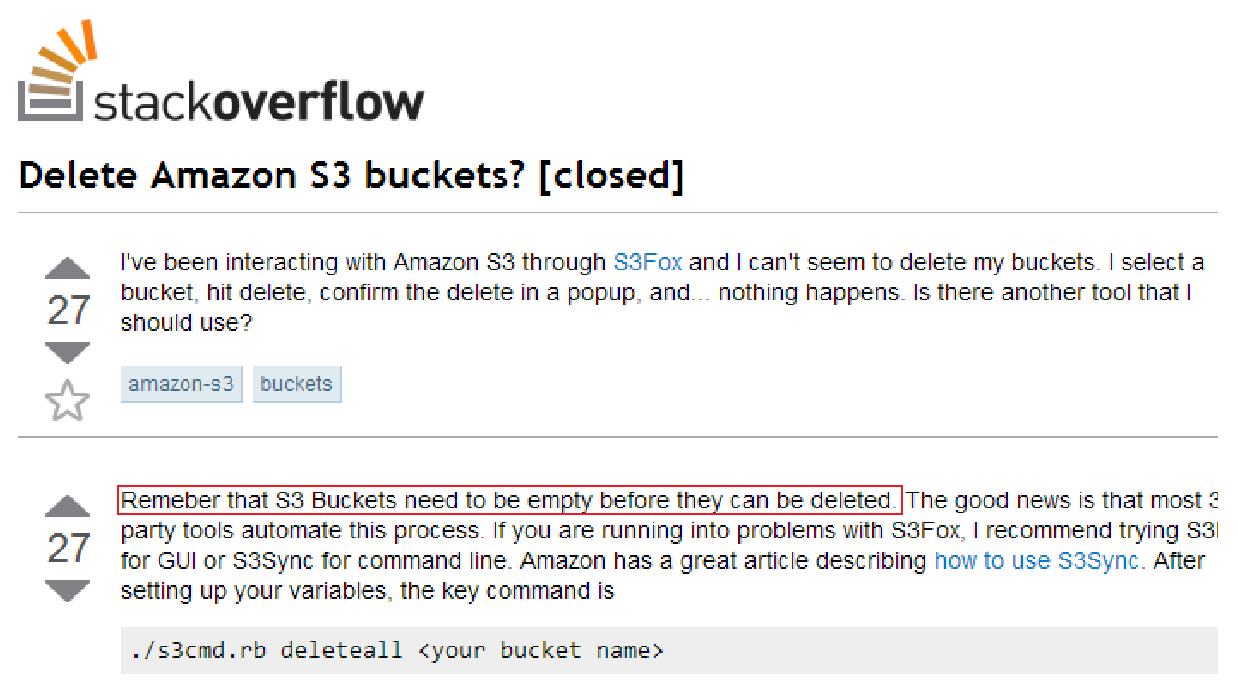
\includegraphics[scale=0.4]{Stackoverflow.eps}
\end{center}
\caption{\label{fig:Stackoverflow} The Query posted on Stackoverflow form regrading Amazon S3 REST API}
\end{figure}

Consider the question asked in \textit{Stack Overflow}~\footnote{\url{http://stackoverflow.com/}} as shown in Figure~\ref{fig:Stackoverflow}. Stack Overflow is a question and answer site for professional and enthusiast programmers. The query is about the delete functionality of a third-party software \CodeIn{S3Fox} to interact with \amazonAPI. In particular, the query complains about an issue in delete bucket functionality of the \CodeIn{S3Fox}. In particular, the issue was because the \CodeIn{S3Fox} developers overlooked the specifications in \amazon. Figure~\ref{fig:AmzonS3DeleteBucketAPI} shows the documentation of delete bucket method. The documents states (outlined in red for clarity) that before deleting the bucket the objects in the buckets must be deleted. Although the issue was fixed but notice that one of the responses on the \textit{Stack Overflow} encouraged the person asking query to switch to another product, thus potentially resulting in a loss of revenue attributed to customer dissatisfaction. In yet another example a developer points out the financial losses he suffered because he was incorrectly using the previously described delete bucket functionality as shown in Figure~\ref{fig:example2}. 


\begin{figure}[t]
\begin{center}
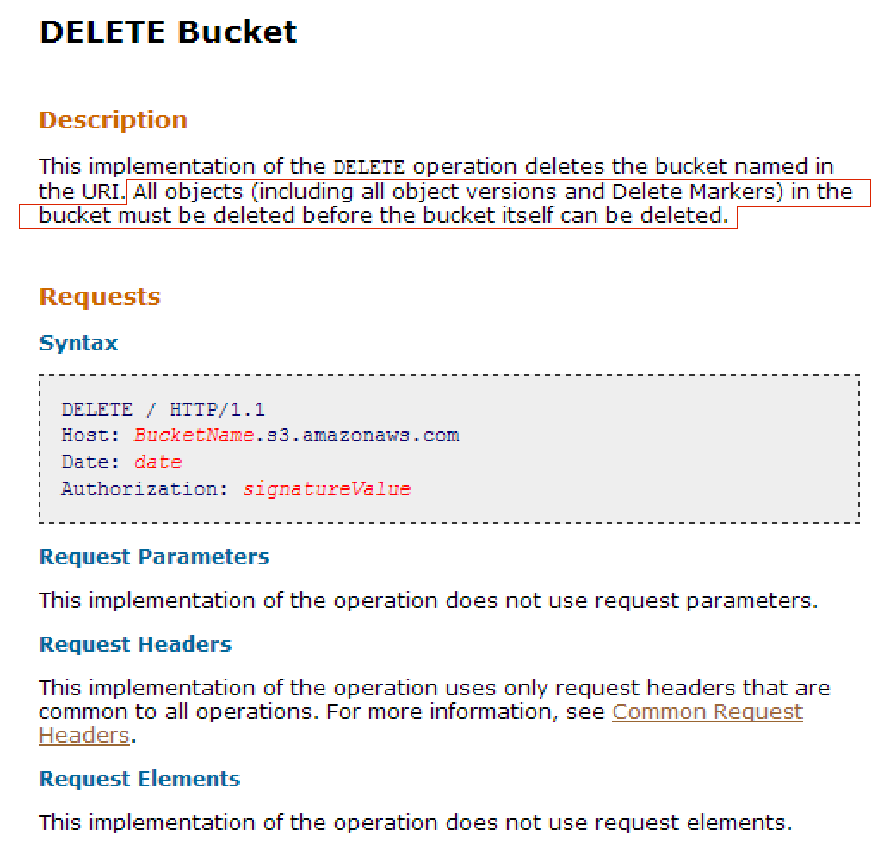
\includegraphics[scale=0.4]{AmzonS3DeleteBucketAPI.eps}
\end{center}
\caption{\label{fig:AmzonS3DeleteBucketAPI} The online API document for \CodeIn{DELETE Bucket} operation in Amazon S3 REST API}
\end{figure}

Formal verification tools can be used to find such kind of defects. However, formal analysis
tools are not designed to work on specifications in natural languages (such as API Documents) and require the specifications in a more formal machine understandable form. 
Thus, there is need for an approach to translate the constraints described in natural language into a more formal notation. In next section, we briefly discuss the related work in this area.


\begin{figure}[t]
\begin{center}
\includegraphics[scale=0.4]{Example2.eps}
\end{center}
\caption{\label{fig:example2} The experience article posted by a developer regarding Amazon S3 REST API}
\end{figure}


 









\section{Related work}
\label{sec:related}

{\small $\bullet$} \textbf{Formal Specification}:
Contracts formally specify the program behavior in terms of conditions that must hold before/after and/or during the execution of a method.
A significant amount of work has been done in automated inference of contracts.
Existing approaches use program analysis~\cite{csallner08dysy,NimmerE02:ISSTA,Tillmann:2006:DLM:2105385.2105433}
to automatically infer contracts.
However, studies~\cite{Polikarpova2009ISSTA,Flanagan2001:HAA} demonstrate that a combination of developer-written and automatically extracted
contracts is the most effective approach for formally specifying the constraints on an API.

Additionally, contracts are typically in the form of assertions on the state (member variables/ properties) of a program. In contrast, temporal constraints specify the ordering of method invocations, therefore are different.
Furthermore, since \tool\ infers temporal constraints from API documents, we envision \tool\ to work in conjunction with existing approaches
to infer a comprehensive formal specification.
 
Another set of approaches infer code-contract-like specifications (such as behavioral model, algebraic specifications, and exception specifications) either dynamically\cite{Henkel07discoveringdocumentation,Ghezzi:2009:SIB:1555001.1555057,Henkel:2008:DDA:1363102.1363105} or statically~\cite{Flanagan2001:HAA,Buse:2008:ADI:1390630.1390664,wasylkowski2011mining} from source code and binaries. 
Among mining based approaches Gable and Su~\cite{gabel2008javert} proposed to learn  
\textit{micro-patterns} of temporal properties from runtime traces and then combining them into larger specifications depicted as finite state automata.
In contrast, \tool\ infers specifications from the natural language text in API documents,
thus complementing existing approaches when the source code or binaries of the API library is not available.


{\small $\bullet$} \textbf{NLP in Software Engineering (SE)}:
Research advances~\cite{Marneffe08COLING,KleinNIPS03} in the accuracy of existing NLP techniques have inspired researchers and practitioners~\cite{pandita12:inferring, pandita13:WHYPER, johnSlankasPASSAT13, XiaoFSE2012, thummalapentaICSE12} to adapt and(/or) apply NLP techniques to solve problems in SE domain. 
Tan et al.~\cite{TanSOSP07} were the first to apply ML and NLP on code comments to detect mismatches between the comments and the implementation.
They rely on predefined rule templates targeted towards threading and lock related comments, and then apply ML-based approach to find comments following such rules.
The constraints inferred by their approach are the restrictions imposed by the developer on the client code.
In comparison, the temporal constraints inferred by \tool\ are the restriction imposed by the API library being used by the client code.

Zhong et al.~\cite{zhong09SE} also leverage ML along with type information to infer constraints on resources from API documents.
Specifically, their approach infers resource constraints following the template - ``\textit{resource creation methods} followed by \textit{resource manipulation methods} followed by \textit{resource release methods}''.
However, temporal constraints are often not be limited to such template. 
Furthermore, the these approaches rely on specific templates for inferring constraints. In contrast, \tool\ works independent of such templates for identifying constraints.


Xiao et al.~\cite{XiaoFSE2012} and Slankas et al.~\cite{johnSlankasPASSAT13} use shallow parsing techniques to infer Access Control Policy (ACP) rules from natural language text in use cases. In contrast, the \tool\ approach works with API documents.
Our previous work~\cite{pandita12:inferring} proposed an NLP-based approach on inferring parameter constraints from method descriptions in the API documents. \tool\ differs from previous work as follows.
\tool\ addresses the problem of inferring temporal constraint, which is not addressed by the previous approach. \tool\ significantly extends the infrastructure in following dimensions.
First, \tool\ relies on ML to identify the temporal constraint sentences. The lower frequency of occurrence of temporal constraint sentences in comparison to parameter constraint sentences, make them harder to detect.
Second, the \tool\ approach introduces hybrid shallow parsing that relies both on parts-of-speech tags as well as Stanford-typed dependencies to construct intermediate representation, while the previous approach relies only on parts-of-speech tags.
Finally, the \tool\ approach leverages the concept of semantic graphs constructed from class and method names in API to automatically infer the implicit method references in a sentence. 


{\small $\bullet$} \textbf{Augmented Documentation}:
Dekel and Herbsleb~\cite{Dekel2009}, were the first to create a tool namely eMoose,
an Eclipse IDE based plug-in that allowed developers to create directives
(way of marking the specification sentences) in the default API documentation.
These directives are highlighted whenever they are displayed in the Eclipse environment.
Lee et al.~\cite{lee2012towards} improved upon their work by providing a formalism to the directives proposed by Dekel et al.~\cite{Dekel2009},
thus allowing tool-based verification.
However, a developer has to manually annotate such directives.
In contrast, \tool\ both identifies the sentences pertaining to temporal constraints and infers the temporal constraints automatically.
\section{Background}
\label{sec:background}

Although, well suited for human communication, converting natural language into unambiguous specifications that can be processed and understood by computers is very difficult.  Recently, a lot of exciting work has been carried out in the area of Natural Language Processing (NLP), with existing NLP techniques proving to be fairly accurate in highlighting grammatical structure of a natural language sentence. However, existing NLP techniques are still in the processing phase and not in understanding phase.  We briefly introduce the NLP techniques used in this work.


\textbf{Parts Of Speech (POS) tagging}~\cite{Klein03,KleinNIPS03}. Also known as \textit{`word tagging'}, \textit{`grammatical tagging'} and \textit{`word-sense disambiguation'}, these techniques aim to identify the part of speech (such as noun, verbs, etc.), a particular word in a sentence belongs to. The most commonly used technique is to train a classification parser over a previously known data set. Current state of the art approaches been have demonstrated to achieve 97\%~\cite{SNLP1} accuracy in classifying POS tags for well written news articles.

\textbf{Phrase and clause parsing}. Also known as chunking, this technique divides a sentence into a constituent set of words (or phrases) that logically belong together (such as a Noun Phrase and Verb Phrase). Chunking thus further enhances the syntax of a sentence on top of POS tagging. Current state-of-the-art approaches can achieve around 90\%~\cite{SNLP1} accuracy in classifying phrases and clauses over well written news articles.

\textbf{Typed Dependencies}~\cite{Marneffe06LREC,Marneffe08COLING}. The Stanford typed dependencies representation  is designed to provide a simple description of grammatical relationships directed towards non-linguistics experts to perform NLP related tasks. It provides a hierarchical structure for the dependencies with precise definitions of what each dependency means, thus facilitating machine based manipulation of natural language text.

\textbf{Named Entity Recognition}~\cite{Finkel05ACL}. Also known as \textit{`entity identification'} and \textit{`entity extraction'}, these techniques are a subtask of IE that aims to classify words in a sentence into predefined categories such as names, quantities, expression of times, etc. These techniques help in associating predefined semantic meaning to a word or a group of words (phrase), thus facilitating semantic processing of named entities. 

\textbf{Co-reference Resolution}~\cite{RaghunathanEMNLP10,LeeCoNLL11}. Also known as \textit{`anaphora resolution'}, these techniques aim to identify multiple expressions present across (or within) the sentences, that point out to the same thing or \textit{`referant'}. These techniques are useful for extracting information; especially if the information encompasses many sentences in a document. 
\section{\tool\ Design}
\label{sec:approach}
%\vspace{-2mm}

\begin{figure}
	\centering
		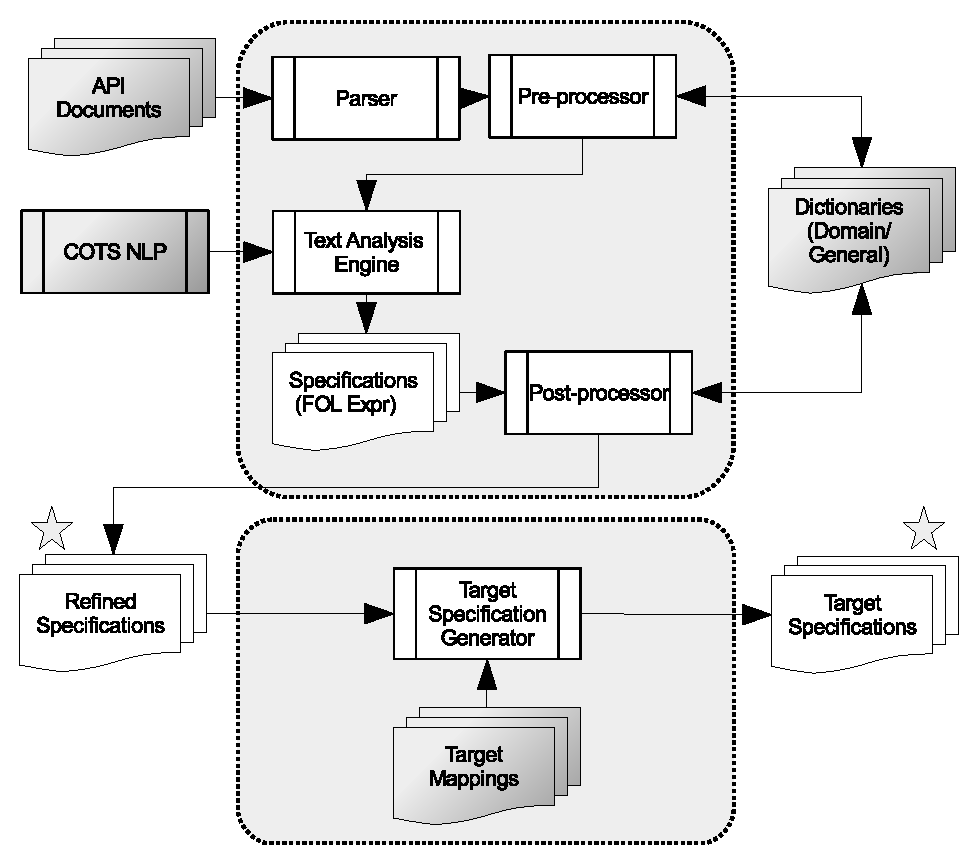
\includegraphics[scale=0.45]{approach.eps}
	\caption{Overview of \tool\ approach}
	\label{fig:approachOverview}
\end{figure}

We next present our approach for inferring specifications from the method descriptions in API Documents.
Figure~\ref{fig:approachOverview} gives an overview of our approach.
Our approach consists of five major components: a preprocessor, a text-analysis engine, a semantic graph generator, specification extractor, and a type analyzer.

The preprocessor accepts API documents and preprocesses the sentences in the method description, such as annotating sentence boundaries and reducing lexical tokens.
The text-analysis engine accepts the pre-processed sentences and annotates them using an NLP parser.
The text-analysis engine further transforms the annotated sentences into the first-order-logic (FOL) representation.
Finally, the specification extractor then leverages the semantic graphs to infer temporal constraints from the FOL representation of a sentence.
Besides the previously described components the approach also consists of a semantic graph generator and type analyzer.
The semantic graph generator accepts the API documents and generates the semantic graphs that are leveraged by specification extractor component.
The type analyzer components infers temporal constraints encoded in the type system of a language by analyzing the API methods parameter and return types.
We next describe each component in detail.


\subsection{Preprocessor}
\label{sub:prep}

The preprocessor accepts the API documents and first extracts method descriptions from it.
In particular, the preprocessor extracts the following fields within method descriptions: 
1) \textit{Summary of the API method},
2) \textit{Summary and type information of parameters of the API method}, 
3) \textit{Summary and type information of return values of the method}, and
4) \textit{Summary and type information of exceptions thrown by the methods}.

This step is required to extract the desired descriptive text from the various presentation styles of the API documents.
In particular, different API documents may have different styles of presenting information to developers.
This difference in style may include the difference in the level of detail presented to the developer.
Our approach thus relies on only basic fields that are trivially available for API methods across different presentation styles. 

After extracting desired information, the natural language text is further preprocessed to be analyzed by subsequent components.
The preprocessing steps are required to increase the accuracy core NLP techniques (described in Section~\ref{sub:CoreNLPback}) that are used in the subsequent phases of \tool\ approach.
In particular, the preprocessor first employs the noun boosting followed by heuristics listed under lexical token reduction, as introduced in Section~\ref{sub:SENLPback}.

Although the previous techniques and heuristics significantly lower the number of lexical tokens in a sentence, some sentences may still contain a considerable number of lexical tokens to overwhelm the POS tagger.
To address this issue, we propose a novel technique (\textit{`Frequent Phrases Reduction'}) to further reduce the number of lexical tokens in a sentence by annotating frequent phrases as a single lexical unit.

In particular, we use n-gram based approach as means to achieve this reduction. 
In the fields of computational linguistics and probability, an n-gram is a contiguous sequence of n words from a given sequence of text or speech. 
We first calculate the most frequently occurring n-grams in the text body. 
In particular, we are interested in the n-grams of length 4 or greater to achieve a reasonable reduction. 
We then prune the list of n-grams based on a subsumption. 
We consider a n-gram of length k ($n_k$) to subsume n-gram of length k-1 ($n_{k-1}$) iff $n_{k-1}$ is a substring of ($n_k$) and the frequency of occurrence of $n_{k-1}$ equals frequency of occurrence of $n_{k}$.
Finally, we rank the list of n-grams based on the frequency of their occurrence in the text, and select top-k n-grams for reduction.
For instance, \textit{Amazon Simple Storage Service}, \textit{an I/O Error Occurs}, and \textit{end of stream} are the examples of such n-grams detected by our approach.
 

%\begin{figure}[t]
%\begin{CodeOut}
%\begin{alltt}
%01: 
%04:
%\end{alltt}
%\end{CodeOut}\vspace*{-2ex}
%\caption{\label{fig:methodAPI} The method description of the \CodeIn{DefineObjectProperty} method in Facebook API}\vspace*{-4ex}
%\end{figure}

\textbf{Prototype Implementation}

Currently our prototype implementation works with online \amazon\ and JDK API. 
However, almost all of the developer documents are provided online as structured webpages.
Thus, current implementation of preprocessor can be easily extended to extract the desired information from any API developer documents.    

Additionally, in current implementation we have manually built the domain dictionaries for the preprocessing using the glossary of terms collected from the websites pertaining to REST and Java API.
We further leveraged the HTML style information in \amazon\ to look for words that were highlighted in code like format. We further leveraged WordNet to maintain a static lookup table of shorthand words to aid named entity handling and abbreviation handling. 

 
Finally, to achieve  n-gram reduction we used Apache Lucene$^{\textregistered}$~\cite{lucene} to achieve.
Apache Lucene is a high-performance, full-featured text search engine library written entirely in Java.
It is a technology suitable for nearly any application that requires full-text search, especially cross-platform.

%Although a POS tagger can be retrained to achieve these pre-processing steps, we prefer annotations to make our approach independent of any specific NLP infrastructure, thus ensuring interoperability with various POS taggers.
	
\subsection{NLP Parser}


The NLP parser accepts the pre-processed documents and annotates every sentence within each document using core NLP techniques described in Section~\ref{sub:CoreNLPback}.
From an implementation perspective, we chose the Stanford parser~\cite{Manning:01}.
However, this component can be implemented using any other existing NLP libraries or approachs.
In particular, we annotate each sentence with POS tags, named-entity Annotations and Stanford-typed dependencies.
For more details on these techniques and their application, please refer to ~\cite{Marneffe06LREC, Marneffe08COLING, pandita12:inferring, pandita13:WHYPER, thummalapentaICSE12}.

%\begin{figure}
%	\centering
%%		\includegraphics[scale=0.6]{StanfordAnnotated.eps}
%	\caption{Sentence annotated with Stanford dependencies}
%	\label{fig:standep}
%\end{figure}
%
%Next we use an example to illustrate the annotations added by the NLP Parser. Consider the example sentence \textbf{\textit{``Also you can share the yoga exercise to your friends via Email and SMS.''}}, that indirectly refers to the READ\_CONTACTS permission. Figure~\ref{fig:standep} shows the sentence annotated with Stanford-typed dependencies. The words in red are the names of dependencies connecting the actual words of the sentence (in black). Each word is followed by the Part-Of-Speech (POS) tag of the word (in green). For more details on Stanford-typed dependencies and POS tags, please refer to ~\cite{Marneffe06LREC,Marneffe08COLING}.

\subsection{Text Analysis Engine}
\label{sub:TAE}
%
%\begin{figure}
%	\centering
%	%	\includegraphics[scale=0.65]{taeRep.eps}
%	\caption{First-order logic representation of annotated sentence in Figure~\ref{fig:standep}}
%	\label{fig:FOLRep}
%\end{figure}

The text analysis engine component accepts the annotated documents and creates an intermediate representation of each sentence.
We define our representation as a tree structure that is essentially a First-Order-Logic (FOL) expression.
Research literature provides evidence of the adequacy of using FOL for NLP related analysis tasks~\cite{Sinha2009,Sinha2010,pandita12:inferring, pandita13:WHYPER}.

In our representation, every node in the tree except for the leaf nodes is a predicate node. 
The leaf nodes represent the entities.
The children of the predicate nodes are the participating entities in the relationship represented by the predicate.
The first or the only child of a predicate node is the governing entity and the second child is the dependent entity.
Together the governing entity, predicate and the dependent entity node form a tuple.  


As described in Section~\ref{sub:SENLPback} the intermediate representation generation technique is based on the principle of shallow parsing~\cite{Branimir2000}. 
In particular, the intermediate-representation technique is implemented as a function of Stanford-typed dependencies~\cite{Marneffe06LREC,Marneffe08COLING,SNLP,KleinNIPS03}, to leverage the semantic information encoded in Stanford-typed dependencies.


However, we observed that such implementation is overwhelmed by complex sentences.
This limitation mandates the use of additional novel technique of \textit{`Frequent Phrases Reduction'} in preprocessing phase.
We further improve the accuracy of intermediate-representation generation by proposing an hybrid approach, i.e. taking into consideration both the POS tags as well as Stanford-typed dependencies.
The POS tags which annotate the syntactical structure of a sentence are used to further simplify the constituent elements in a sentence. 
We then use the Stanford-typed dependencies that annotate the grammatical relationships between words to construct our FOL representation.
Thus, the intermediate representation generator used in this work is two phase process as opposed to previous work~\cite{pandita12:inferring, pandita13:WHYPER}. 
We next describe these two phases:

\textbf{POS Tags}: We first parse a sentence based on the function of POS tags. 
In particular, we use semantic templates to logically break a sentences into smaller constituent sentences. 
For instance, consider the sentence:

\begin{center}
\scriptsize``All objects (including all object versions and Delete Markers) in the bucket must be deleted before the bucket itself can be deleted.''. \normalsize
\end{center}

The Stanford parser inaccurately annotates the Stanford-typed dependencies of the sentence because of presence of different clauses acting on different subject-object pairs.
We thus break down the sentence into two smaller tractable sentences:

\begin{center}
\scriptsize \textit{``All objects in the bucket must be deleted before the bucket itself can be deleted.}''
	
\textit{``All objects including all object versions and Delete Markers.''}\normalsize 
\end{center} 


Table~\ref{tab:semanticTemplates} shows a list the semantic templates used in this phase.
Column ``Template'' describes conditions where the template is applicable and Column ``Summary'' describes the action taken by our shallow parser when the template is applicable.
All of these semantic templates are publicly available on our project website~\cite{projectweb}.
With respect to the previous example the template no. 3 \textit{( A noun phrase followed by another noun/pronoun/verb phrase in brackets)} is applicable.
Thus our shallow parser breaks the sentence into two individual sentences.
	 
\textbf{Stanford-typed Dependencies}: This phase is equivalent to the intermediate-representation technique described in Section~\ref{sub:SENLPback}.

\subsection{Specification Extractor}
\label{sub:SE}

This component accepts the FOL representation of the sentence.

\begin{itemize}
\item Extracts Specifications from FOL representation. 
\item Specifically looking for modal modifies ``can, could, may, must, should'' 
\item Takes into consideration the negative quantifiers.
\item Algorithm to infer the sequence of operations.
\end{itemize}


\begin{table*}
\begin{center}

\caption{Semantic Templates}
    \begin{tabular}{ | l | p{5cm} |p{10cm} |}
    \hline
    \textbf{S No.} 	& \textbf{Template} & \textbf{Summary} \\ \hline
    
    1. 		& Two sentences joined by a conjunction & Sentence is broken down into two individual sentences with the conjunction term serving as the connector between two. \\ \hline
    2. 		& Two sentences joined by a ``,''& Sentence is broken down to individual independent sentences \\ \hline
    3.		& A noun phrase followed by another noun/pronoun/verb phrase in brackets & Two individual sentences are formed. The first sentence is  the same as the parent sentence sans the noun/pronoun.verb phrase in bracket. The second sentence constitutes of the noun phrase followed by  noun/pronoun/verb phrase without the brackets.\\ \hline
    4.		& A noun phrase by a conditional phrase in brackets & Two individual sentences are formed. The first sentence is the same as the parent sentence sans the conditional phrase in bracket. The second sentence constitutes of noun phrases followed by conditional in the bracket.\\ \hline
    5.		& A conditional phrase followed by a sentence & Two dependent sentences are formed. The first sentence constitutes the conditional phrase. The second sentence constitutes rest of the sentence.\\ \hline
    6.		& A sentence in which the parent verb phrase is over two child verb phrases joined by a conjunction & Two dependent sentences are formed where the dependency is the conjunction. The first sentence is formulated by removing conjunction and second child verb phrase. The second sentence is formulated by removing conjunction and first child verb phrase. \\ \hline
    \end{tabular}
	\label{tab:semanticTemplates}
\end{center}
\end{table*}


\subsection{Semantic-Graph Generator}
\label{sub:ACA}

A key way of identifying reference to a method within the API in our proposed approach is the employment of a semantic graph of an API.
In particular, we propose to initially infer such graphs from API documents.
Manually creating a semantic graph is prohibitively time consuming and may be error prone.
We thus employ a systematic methodology (proposed previously in ~\cite{pandita13:WHYPER}) to infer such semantic graphs from API documents that can potentially be automated.
We first consider the name of the class.
We then find the synonyms terms used refer to the class in question.
The synonym terms are listed as by breaking down the camel-case notation in the class name.
This list is further augmented by listing the name of the parent classes and implemented interfaces if any. 

\begin{figure}
	\centering
		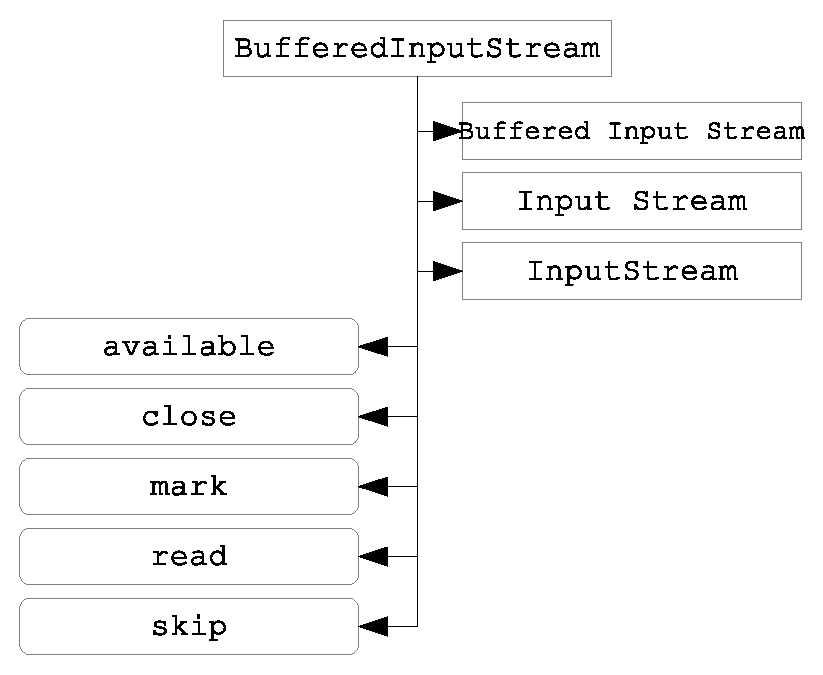
\includegraphics[scale=0.4]{KnowledgeGraph.eps}
	\caption{Semantic Graph for the \CodeIn{BufferedInputStream} class in Java}
	\label{fig:knowledge}
\end{figure} 


We then systematically inspect the member methods to identify actions applicable to the objects represented by the class. From the name of a public method (describing a possible action on the object), we extract verb phrases. The verb phrases are used as the associated actions applicable on the object. For instance, \CodeIn{BufferedInputReader} defines operations available, close, mark, and so on. We associate these operations with the objects of type \CodeIn{BufferedInputReader}. Figure~\ref{fig:knowledge} shows a sub-graph of  graph for \CodeIn{BufferedInputReader} class. The phrases in solid rectangles are synonyms of the class name \CodeIn{BufferedInputReader}. The phrases in rounded rectangle are the actions applicable on \CodeIn{BufferedInputReader} class.
  


\algsetup{indent=1em}
\begin{algorithm}[t!]
\begin{algorithmic}[1]
\begin{scriptsize}
\REQUIRE K\_Graph $g$, FOL\_rep $rep$ 
\ENSURE String $action$
\STATE $String\ action\ =\ \phi$
\STATE $List\ r\_name\_list\ =\ g.resource\_Names$
\STATE $FOL\_rep\ r'\ =\ rep.findLeafContaining(r\_nam\_list)$
\STATE $List\ actionList\ =\ g.actionList$
\WHILE{$(r'.hasParent)$}
	\IF{$actionList.contains(r'.parent.predicate)$}
		\STATE $action\ =\ actionList.matching(r'.parent.predicate)$
		\STATE $break$
	\ELSE
		\IF{$actionList.contains(r'.leftSibling.predicate)$}
			\STATE $action\ =\ actionList.matching(r'.leftSibling.predicate)$
			\STATE $break$
		\ENDIF
	\ENDIF
	\STATE $r'\ =\ r'.parent$
\ENDWHILE
\RETURN $action$
\end{scriptsize}
\end{algorithmic}
\caption{Action\_Extractor}
\label{alg:SenAnnotaator}
\end{algorithm} 


\begin{algorithm}[t!]
\begin{algorithmic}[1]
\begin{scriptsize}
\REQUIRE List $methodList$ 
\ENSURE Graph $seq\_Graph$
\STATE $Graph\ seq\_Graph\ =\ \phi$
\STATE $Map\ idx\ = createIdx(methodList)$

\FORALL{$Method\ mtd\ in\ methodList$} 
	\STATE $seq\_Graph.addVertex(mtd)$
\ENDFOR

\FORALL{$Method\ mtd\ in\ methodList$} 
	\IF{$mtd.isPublic()$}
		\IF{$!mtd.isStatic()$}
			\STATE $List\ preList\ =\ idx.query(mtd.declaringType)$
			\FORALL{$Method\ mtd'\ in\ preList$}
				\STATE $seq\_Graph.addEdge(mtd',mtd)$
			\ENDFOR
		\ENDIF
		\FORALL{$Parameter\ param\ in\ mtd.getParameters()$}
			\IF{$!isBasicType(param.Type)$}
				\STATE $List\ preList\ =\ idx.query(paramType)$
				\FORALL{$Method\ mtd'\ in\ preList$}
					\STATE $seq\_Graph.addEdge(mtd',mtd)$
				\ENDFOR				
			\ENDIF
		\ENDFOR
	\ENDIF
\ENDFOR
\RETURN $seq\_Graph$
\end{scriptsize}
\end{algorithmic}
\caption{Type\_Sequence\_Builder}
\label{alg:SeqAnnotaator}
\end{algorithm} 



%The FOL representation helps us effectively deal with the problem of \emph{confounding effects} of keywords as described in Section~\ref{sec:overview}. In particular, the FOL assists in distinguishing between a resource that would be a leaf node and an action that would be a predicate node in the intermediate representation of a sentence. The generated FOL representation of the sentence is then provided as an input to the semantic engine for further processing.
%
%
%
%\subsection{Semantic Engine (SE)}
%\label{sub:SE}
%The Semantic Engine (SE) accepts the FOL representation of a sentence and based on the semantic graphs of Android permissions annotates a sentence if it matches the criteria. A semantic graph is basically a semantic representation of the resources which are governed by a permission. For instance, the READ\_CONTACTS permission governs the resource ``CONTACTS'' in Android system.
%
%
%Figure~\ref{fig:knowledge} shows the semantic graph for the permission READ\_CONTACTS. A semantic graph primarily constitutes of subordinate resources of a permission (represented in rectangular boxes) and a set of available actions on the resource itself (represented in curved boxes). Section~\ref{sub:ACA} elaborates on how we build such graphs systematically.
%
%Our SE accepts the semantic graph pertaining to a permission and annotates a sentence based on the algorithm shown in Algorithm~\ref{alg:SenAnnotaator}. The Algorithm accepts the FOL representation of a sentence $rep$, the semantic graph associated with the resource of a permission $g$ and a boolean value $recursion$ that governs the recursion. The algorithm outputs a boolean value $isPStmt$, which is \CodeIn{true} if the statement describes the permission associated with a semantic graph ($g$), otherwise \CodeIn{false}. 
%
%Our algorithm systematically explores the FOL representation of the sentence to determine if a sentence describes the need for a permission. First, our algorithm attempts to locate the occurrence of associated resource name within the leaf node of the FOL representation of the sentence (Line 3). The method \CodeIn{findLeafContaining(name)} explores the FOL representation to find a leaf node that contains term \CodeIn{name}. Furthermore, we use WordNet and Lemmatisation~\cite{Do09:Robust} to deal with synonyms of a word in question to find appropriate matches. Once a leaf node is found, we systematically traverse the tree from the leaf node to the root, matching all parent predicates as well as immediate child predicates [Lines 5-16].
%
%Our algorithm matches each of the traversed predicate with the actions associated with the resource defined in semantic graph. Similar to matching entities, we also employ WordNet and Lemmatisation~\cite{Do09:Robust} to deal with synonyms to find appropriate matches. If a match is found, then the value \CodeIn{isPStmt} is set to  \CodeIn{true}, indicating that the statement describes a permission.
%
%In case no match is found, our algorithms recursively search all the associated subordinate resources in the semantic graph of current resource. A subordinate resource may further have its own subordinate resources. Currently, our algorithm considers only immediate subordinate resources of a resource to limit the false positives.
%
%%We limit the exploration to depth 1 to limit the false positives. That means only immediate subordinate resources of a resource will be explored.
%
%In the context of the FOL representation shown in Figure~\ref{fig:FOLRep}, we invoke Algorithm~\ref{alg:SenAnnotaator} with the semantic graph shown in Figure~\ref{fig:knowledge}. Our algorithm attempts to find a leaf node containing term ``CONTACT'' or some of its synonym. Since the FOL representation does not contain such a leaf node, algorithm calls itself with semantic graphs of subordinate resources (Line 17-25), namely `NUMBER', `EMAIL', `LOCATION', `BIRTHDAY', `ANNIVERSARY'. 
%
%The subsequent invocation will find the leaf-node ``email'' (annotated 9 in Figure~\ref{fig:FOLRep}). Our algorithm then explores the preceding predicates and finds predicate ``share'' (annotated 2 in Figure~\ref{fig:FOLRep}). The Algorithm matches the word ``share'' with action ``send'' (using Lemmatisation and WordNet similarity), one of the actions available in the semantic graph of resource `EMAIL' and returns \CodeIn{true}. Thus, the sentence is appropriately identified as describing the need for permission READ\_CONTACT. 
%
%


\section{Evaluation}
\label{sec:evaluation}

We conducted an evaluation to assess the effectiveness of \tool. In our evaluation, we address two main research questions:

\begin{itemize}
	\item\textbf{RQ1}: What are the precision and recall of \tool\  in
	identifying temporal constraints from sentences written in natural language?
	\item\textbf{RQ2}: What is the accuracy of \tool\ in inferring temporal constraints from specification sentences in the API documents?
	\item\textbf{RQ3}: How do the constraints inferred by our approach compare with the typed-enforced temporal constraints?
 
\end{itemize}

\subsection{Subjects}
\label{sub:subject}

We used the API documents of the following two libraries as subjects for our evaluation. 
\begin{itemize}
	\item{Amazon S3}. \amazon\ provides a REST based web services interface that can be used to store and retrieve data on the web. Furthermore, \CodeIn{Amazon S3} also empowers a developer with rich set of API methods to access a highly scalable, reliable, secure, fast, inexpensive infrastructure. \CodeIn{Amazon S3} is reported to store more than 2 trillion objects as of April 2013 and gets over 1.1 million requests per second at peak time~\cite{amazons3stats}.

	\item{java.io}. \CodeIn{java.io} is a popular packacge in \CodeIn{Java} programming language that provides APIs for system input and output through data streams, serialization and the file system.
\end{itemize}
We chose \CodeIn{Amazon S3} and \CodeIn{java.io} APIs as our subjects because they are popular and contain decent documentation.

\subsection{Experimental Setup.} 
We first manually annotated the sentences in the API documents of the two APIs.
Two authors manually labeled each sentence in the API documentation as sentence containing 
temporal constraints or not.
We used \CodeIn{cohen kappa}~\cite{carletta1996assessing} score to statistically measure
the inter-rater agreement.
The \CodeIn{cohen kappa} score of the two authors was .66 (on a scale of 0 to 1), 
which denotes a statically significant agreement. 
After the authors classified all the sentences, they 
discussed with each other to reach a consensus on the sentences they classified differently. 
We use this classified sentences as the golden set for calculating precision and recall.

 


To answer RQ1, we measure the number of true positives ($TP$), false positives ($FP$), true negative ($TN$), and false negatives ($FN$)
in identifying the specification sentences by \tool.
We define specification sentence as a sentence describing a temporal constraints.
We define the $TP$, $FP$, $TN$, and $FN$ of \tool\ as follows:

\begin{enumerate}
	\item $TP$: A sentence correctly identified by \tool\ as specification sentence.
	\item $FP$: A sentence incorrectly identified by \tool as specification sentence.
	\item $TN$: A sentence correctly identified by \tool\ as not a specification sentence.
	\item $FN$: A sentence incorrectly identified by \tool\ as not a specification sentence.
\end{enumerate}


In statistical classification~\cite{Olson08}, $Precision$ is defined as a ratio of
number of true positives to the total number of items reported to be true,
$Recall$ is defined as a ratio of number of true positives to the total number
of items that are true. $F-score$ is defined as the weighted harmonic mean of 
$Precision$ and $Recall$. Higher value of $Precision$, $Recall$, and $F-Score$
are indicative of higher quality of the specification statements inferred using 
\tool. based on the calculation of $TP$, $FP$, $TN$, and $FN$ of \tool\ defined
previously we computed the $Precision$, $Recall$, and $F-Score$ of \tool\ as follows:


\begin{center}

$Precision$ = $\frac{TP}{TP + FP}$

$Recall$ = $\frac{TP}{TP + FN}$

$F-Score$ = $\frac{2 X Precison X Recall}{Precision + Recall}$
\end{center}


To answer RQ2, we checked the temporal constraints inferred from specification sentences by \tool.
We measure $accuracy$ of \tool as the ratio of the total number of temporal constraints that
are correctly inferred by \tool to the total number of specification sentences. 

\subsection{Results}

We next describe our evaluation results to demonstrate the effectiveness of \tool\ in identifying temporal constraints.

\begin{table*}
\begin{center}

\caption{Evaluation Results}

\begin{tabular}{|c|c|c|c|c|c|c|c|c|c|c|}
\hline API & Methods & Sentences & Spec Sentences & \tool\ Ann & TP & FP & FN & P(\%) & R(\%) & F-Score(\%) \\
\hline 
\hline java.io &  & 2417 & 78 & 88 & 57 & 31 & 21 & 64.8 & 73.1 & 68.8 \\ 
\hline AMAZON S3 REST & 51 & 1492 & 12 & 12 & 8 & 4 & 4 & 66.7 & 66.7 & 66.7 \\ 
\hline Total &  & 3909 & 90 & 100 & 65 & 35 & 25 & 65.0$^*$ & 72.2$^*$ & 68.4$^*$ \\ 
\hline
%----------------- END TABLE DATA ------------------------ 
\multicolumn{11}{p{6.5in}}{\footnotesize $^*$ Column average; TP: Total number of True Positives; 
FP: Total number of False Positives; FN: Total number of False Negatives; P: Precision; R: Recall} \\ 
\end{tabular}
\label{tab:results}
\end{center}
\end{table*}


\subsubsection{RQ1: Effectiveness in Identifying Specification Sentences}


In this section, we quantify the effectiveness of \tool\ in identifying specification sentences by answering RQ1.
Table~\ref{tab:results} shows the effectiveness of \tool\ in identifying specification sentences.
Column ``API'' lists the names of the subject API. 
Column ``Methods'' and ``Sentences'' lists the number of methods and sentences in each subject API's.
Column ``\tool\ Ann'' lists the number of sentences identified by \tool\ as constraint sentences. 
Columns ``TP'', ``FP'', ``TN'', and ``FN'' represent the number of \CodeIn{true positives}, \CodeIn{false positives}, \CodeIn{true negatives}, and \CodeIn{false negatives}, respectively. 
Columns ``P(\%)'', ``R(\%)'', and ``F-Score(\%)'' list percentage values of \CodeIn{precision}, \CodeIn{recall}, and \CodeIn{F-score} respectively. 
Our results show that, out of 3,909 sentences, \tool\ effectively identifies specification sentences with the average precision, recall, and F-score of 65.0\%, 72.2\%, and 68.4\%, respectively.

 

%We next present an example to illustrate how \tool\ incorrectly identifies a sentence as a specification sentence. \textbf{A example goes here}
We next present an example to illustrate how \tool\ incorrectly identifies a sentence as a specification sentence (producing false positives). For instance, consider the sentence ``\textit{This is done by flushing the stream and then closing the underlying output stream.}'' from  \CodeIn{close} method description from \CodeIn{PrintStream} class. \tool\ incorrectly identifies the action ``flush'' being performed before the action ``close''. However \tool\ fails to make the distinction that it happens internally (enforced within the body) in the method. \tool, thus incorrectly identifies the sentence as a specification sentence.   


Another major source of FPs is the incorrect parsing of sentences by the underlying NLP infrastructure and/or inadequacy of generic dictionaries for synonym analysis. For instance, consider the sentence ``\textit{If this stream has an associated channel then the channel is closed as well.}'' from the \CodeIn{close} method description from \CodeIn{FileOutputStream}. The sentence describes an effect that happens as a result of calling the \CodeIn{close} method and does not describe any temporal constraint. However, \tool\ annotates the sentence as a specification sentence because underlying Wordnet dictionaries matches the word ``has'' as a synonym of ``get''. This incorrect matching in turn causes \tool to incorrectly annotate the sentence as specification sentence because ``has'' is matched against \CodeIn(get) method in \CodeIn{FileOutputStream}. We observed 8 instances of previously described example in our results.

If we manually fixed the Wordnet dictionaries to match ``has'' and ``get'' as synonyms, our precision is further increased to 70.8\% effectively increasing the F-Score of \tool to 71.2\%. We refrained from including such modifications for reporting the results to stay true to our proposed framework. In the future, we plan to investigate techniques to construct better domain dictionaries for software API.

We next present an example to illustrate how \tool\ fails identify a specification sentence (producing false negative). False negatives are undesirable in the context of our problem domain, because they can mislead the users of \tool\ into believing that no other temporal constraint exists in the API documents. Furthermore, an overwhelming number of false negatives works against the usefulness of \tool. For instance, consider the sentence ``\textit{This is done by flushing the stream and then closing the underlying output stream.}'' from  \CodeIn{close} method description from \CodeIn{PrintStream} class. The sentence describes the constraint in terms of invoking the same method again. Although \tool\ correctly identifies the method \CodeIn{close} in the sentence, \tool\ currently does not support temporal constraint on the same method. Aforementioned, limitation causes \tool\ to not identify the statement as a specification constraint.   


Another major source of false negatives (similar to reasons for false positives) is the incorrect parsing of sentences by the underlying NLP infrastructure. For instance, consider the sentence ``\textit{If any in-memory buffering is being done by the application (for example, by a BufferedOutputStream object), those buffers must be flushed into the FileDescriptor (for example, by invoking OutputStream.flush) before that data will be affected by sync.}'' The sentence describes that the \CodeIn{OutputStream.flush()} must be invoked before invoking the current method if in-memory buffering is performed. However, the length and complexity in terms of number of clauses causes the underlying Stanford parser to inaccurately annotate the dependencies, which eventually results into incorrect classification. 

Overall, a significant number of false positives and false negatives will be reduced as the current NLP research advances the underlying NLP infrastructure. Furthermore, use of domain specific dictionaries as opposed to generic dictionaries used in current prototype implementation will further improve the precision and recall of \tool. 

\subsubsection{RQ2: Accuracy in Inferring Temporal Constraints}

In this section, we evaluate the effectiveness of \tool\ in inferring specification sentences from API documents.

If any in-memory buffering is being done by the application (for example, by a BufferedOutputStream object), those buffers must be flushed into the FileDescriptor (for example, by invoking OutputStream.flush) before that data will be affected by sync.


If markposMM is -1MM (no mark has been set or the mark has been invalidated), an IOExceptionMM is thrown.

\subsubsection{RQ3: Comparison to Typed-Enforced Constraints}

In this section, we compared the temporal constraints inferred from the natural language API descriptions to those enforced by the type-system. For answering this question we used the constraints inferred by the Algorithm~\ref{alg:TypeAnalysis} presented in Section~\ref{sec:approach} on classes in \CodeIn{java.io} package.

We observed that the constraints inferred by our \tool\ from natural language text were distinct from the constraints enforced by the type system. 



\subsection{Summary}
\label{sub:summary}



\subsection{Threats to Validity}
\label{sub:threats_to_validity}
Threats to external validity primarily include the degree to which the subject documents used in our evaluations are representative of true practice. To minimize the threat, we used API documents of two representative commercial REST API: one dealing with online storage and the other \textbf{TBD}. The \amazon documents describe one of the most popularly used and online storage APIs. We also used the \textbf{TBD}. Furthermore, the difference in the functionalities provided by the two projects also address the issue of over fitting our approach to a particular type of API. The threat can be further reduced by evaluating our approach on more subjects. 

Threats to internal validity include the correctness of our implementation in extracting usage constraints and labelling a statement as a constraint statement. To reduce the threat, we manually inspected all the constraints inferred against the API method descriptions in our evaluation. Furthermore, we ensured that the results were individually verified and agreed
upon by two authors.





\section{Limitations and Future work}
\label{sec:discussion}

Our approach serves as a way to formalize the description of constraints in the natural language texts of API documents, thus facilitating existing tools to process these specifications. We next discuss some of the limitations of our approach.

\textbf{Validation of Method Descriptions}. API documents can sometimes be misleading~\cite{tcomment,Cindy10:PASTE}, thus causing developers to write faulty client code. In future work, we plan to extend our approach to find documentation-implementation inconsistencies.

\textbf{Inferring Implicit Constraints}. The approach presented in this work only infers temporal constraints explicitly described in the method descriptions.
However, there are instances where the constraints are implicit. For instance, consider the method description for \CodeIn{markSupported} method in \CodeIn{BufferInputStream} class in Java, which states ``\textit{Test if this input stream supports \CodeIn{mark}}''. For a developer it is straightforward to understand that the method \CodeIn{markSupported} must be invoked before the method \CodeIn{mark}. Our approach is unable to infer such implicit temporal constraints. In future work, we plan to investigate techniques to infer these implicit temporal constraints.

\textbf{Extending Generic Dictionaries}. The use of generic dictionaries for software engineering related text is sometimes inadequate. For instance, Wordnet matches ``has'' as a synonym for the word ``get''. Although valid for generic English, such instances cause our approach to incorrectly distinguish a constraint sentence from a regular sentence, or vice versa. In future work, we plan to investigate techniques to extend generic dictionaries for software engineering related text. In particular, Yang and Tan~\cite{swordnet} recently proposed a technique for inferring semantically similar words from software context to facilitate code search. We plan to explore such techniques and evaluate the overall effectiveness of our approach after augmenting it with such techniques.  

%\textbf{Bug Finding Capabilities}
%
%
%
%~\cite{lee2012towards} manually wrote specifications for JDK API. One of the evaluations they conducted was to see if the formal representation of the constraints in the natural language in API documents could detect violations. They also used \CodeIn{java.io} as subject API to manually write specifications. 
%
%they used java benchmarks from [S. M. Blackburn, R. Garner, C. Hoffman, et al. The DaCapo benchmarks: Java benchmarking development and analysis. In OOPSLA, 2006.] to detect voilations.
%
%\textit{The error specification, Reader ManipulateAfterClose is violated on all benchmarks but avrora. However, after analyzing the source code, we found that SimpleCharStream intentionally performs a read operation after closing the stream for checking if the stream is closed or not. Also, it handles thrown exceptions properly. There is no bug in this class related to this specification, but this is not a usual pattern of using the Reader class according to the JDK API; the code should probably be changed.}--reproduction of the text from ~\cite{lee2012towards}. Our approach infers this constraint.
%
%Other bug that can be detected is regarding REST API discussed in example section


%
%
%\textbf{Code Searching}. Code searching~\cite{thummalapenta07parseweb,Reiss2009SCS} for reuse is a classic problem~\cite{FrakesIEEETran05} in software engineering. Among previous approaches, a recent approach by Riess~\cite{Reiss2009SCS} provides promising results by using semantics such as code contracts as input-output relationships for code searching. Our approach can be used for generating specifications from API documents in a code repository and thus assisting such approaches in producing better results.
%
%\textbf{Program Synthesis}. Automated program synthesis holds potential for easing the task of a developer by taking care of program generation and allowing the developer to concentrate on design tasks. Recent work by Srivastava et al.~\cite{Srivastava2010PVP} addresses the problem by leveraging specifications in the form of pre/post-conditions and invariants to achieve synthesis. Our approach can work in conjunction with such approaches to extract specifications from natural language text to achieve better synthesis.
%
%\vspace*{-1ex}

 
    



%\textbf{Leveraging Error Descriptions}
%
%\CodeIn{BucketAlreadyExists}: \textit{``The requested bucket name is not available. The bucket namespace is shared by all users of the system. Please select a different name and try again.''}
%
%\textbf{Semantic Flow}


%\vspace*{-1ex}
%
%\textbf{Information flow analysis}. Our approach currently takes into account the specifications described in a single sentence. However, there are instances when a specification is distributed across several sentences. Consider the sentences below:
%
%\begin{center}
% \small{\textit{``parameter values:Id-value pairs of preferences to set. Each id is an integer between 0 and 200 inclusively. Each value is a string with maximum length of 128 characters.''}}
%\end{center}
%
%The first sentence describes the data structure used for the variable values. The sentences following the first sentence describe the specification on each item in the data structure. Since currently our approach works on individual sentences, it is not possible to establish the relationship between the specifications described in later sentences to the first sentence. In future work, we plan to investigate techniques to facilitate information flow analysis to handle such situations.
%
%\textbf{Contextual Information}. Some API documents are not comprehensive. Method descriptions omit certain specifications that have already been described in another closely related method. Currently, our approach does not deal with such scenarios as we do not consider contextual information. In future work, we plan to explore techniques to infer specifications in such scenarios.
%
%
%%Consider the method description from the facebook API:
%
%%\textit{\textbf{``summary:}}
%
%%\textit{Rename a previously defined object type. }
%
%%\textit{\textbf{parameter:obj\_type}:Previous name of the object type to rename.}
%
%%\textit{\textbf{parameter:new\_name:} New name to use. This name needs to be unique among all object types and associations defined for this application. This name also needs to be a valid identifier, which is no longer than 32 characters, starting with a letter (a-z) and consisting of only small letters (a-z), numbers (0-9) and-or underscores.''}
%
%
%%The method description describes the restrictions related to the variable \textit{new\_name}. However, there is no description of specifications related to \textit{obj\_type}. Since the method deals with renaming object types, the restrictions of one the parameters apply on the other. 
%
%%\textbf{Leveraging class descriptions and code-comments:} Currently our approach only takes into account the method descriptions of the API documents. As a result, the extracted specifications are in the form of pre/post conditions. We plan to extend the approach to the class descriptions to extract class invariants~\cite{csallner08dysy}. We further plan to extend our approach to take into account the code comments to generate formal specifications within a method. Leveraging code comments would further benefit the functional verification of a method as demonstrated earlier by Lin Tan et al.~\cite{TanSOSP07}.
%
%\textbf{Elimination of Predefined Lists}. The current implementation of our approach uses predefined lists for domain dictionaries. There are approaches~\cite{Zhou2008} that facilitate building domain dictionaries from source code. We plan to extend our implementation to use these approaches. Furthermore, we rely on pre-defined templates for code contract generation. While such a strategy serves our purpose of prototyping, advanced techniques such as keyword programming~\cite{Little2009} have shown promising results in building programming statements using keywords. We plan to explore such techniques and evaluate the overall effectiveness of our approach after augmenting it with such techniques.
%

\section{Conclusion}
\label{sec:conclusion}
\vspace*{-1ex}
Despite being highly desirable, formal temporal constraints are missing from most APIs.
In contrast, documentation of API methods contains detailed specifications of temporal constraints in natural language text.
Manually writing formal specifications based on natural language text in API documents is prohibitively time-consuming and error-prone.
To address this issue, we have proposed a novel approach called \tool\ to infer temporal constraints from natural language text of API documents.
We used \tool\ to infer temporal constraints from
the \paypalAPI, the \amazonAPI, and the 
commonly used package \CodeIn{java.io} in the JDK API.
Our evaluation results show that \tool\ effectively identifies sentences describing
temporal constraints with an average 79\% precision and 60\% recall,
from more than 4000 sentences in subject API documents.
Furthermore, \tool\ also achieved an accuracy of
70\% in inferring 77 formal temporal constraints from these temporal constraint sentences.

%
% The following two commands are all you need in the
% initial runs of your .tex file to
% produce the bibliography for the citations in your paper.
\bibliographystyle{abbrv}
\bibliography{rahul}  % sigproc.bib is the name of the Bibliography in this case
% You must have a proper ".bib" file
%  and remember to run:
% latex bibtex latex latex
% to resolve all references
%
% ACM needs 'a single self-contained file'!
%
%APPENDICES are optional
%\balancecolumns
%\appendix
%%Appendix A
%\section{Headings in Appendices}
%The rules about hierarchical headings discussed above for
%the body of the article are different in the appendices.
%In the \textbf{appendix} environment, the command
%\textbf{section} is used to
%indicate the start of each Appendix, with alphabetic order
%designation (i.e. the first is A, the second B, etc.) and
%a title (if you include one).  So, if you need
%hierarchical structure
%\textit{within} an Appendix, start with \textbf{subsection} as the
%highest level. Here is an outline of the body of this
%document in Appendix-appropriate form:
%\subsection{Introduction}
%\subsection{The Body of the Paper}
%\subsubsection{Type Changes and  Special Characters}
%\subsubsection{Math Equations}
%\paragraph{Inline (In-text) Equations}
%\paragraph{Display Equations}
%\subsubsection{Citations}
%\subsubsection{Tables}
%\subsubsection{Figures}
%\subsubsection{Theorem-like Constructs}
%\subsubsection*{A Caveat for the \TeX\ Expert}
%\subsection{Conclusions}
%\subsection{Acknowledgments}
%\subsection{Additional Authors}
%This section is inserted by \LaTeX; you do not insert it.
%You just add the names and information in the
%\texttt{{\char'134}additionalauthors} command at the start
%of the document.
%\subsection{References}
%Generated by bibtex from your ~.bib file.  Run latex,
%then bibtex, then latex twice (to resolve references)
%to create the ~.bbl file.  Insert that ~.bbl file into
%the .tex source file and comment out
%the command \texttt{{\char'134}thebibliography}.
%% This next section command marks the start of
%% Appendix B, and does not continue the present hierarchy
%\section{More Help for the Hardy}
%The acm\_proc\_article-sp document class file itself is chock-full of succinct
%and helpful comments.  If you consider yourself a moderately
%experienced to expert user of \LaTeX, you may find reading
%it useful but please remember not to change it.
%\balancecolumns
%% That's all folks!
\end{document}
